\documentclass{beamer}
%%%%%%%%%%%%%%%%%%%%%%%%%%%%%%%%%%%%%%%%%%%%%%%%%%%%%%%%%%%%%%%%%%%%%%%%%%%%
\usepackage{bm}
\usepackage{amsmath}
\usepackage{amssymb}
%\usepackage{microtype}
\usepackage{booktabs} % \toprule, \midrule, \bottomrule
%%% INCLUDE FILE FOR DEFINITIONS
%%% These may require various packages.

% Shortcuts in regular text
\newcommand{\degs}{\ensuremath{^\circ}}
\newcommand{\EE}[1]{\ensuremath{\times 10^{#1}}}
\newcommand{\ttimes}{\ensuremath{{}\times{}}}
\newcommand{\cclicense}{%
  \smash{\raisebox{-0.45ex}{%
  \setlength{\unitlength}{1em}%
  \begin{picture}(1,1)%
    \put(0.5,0.5){\circle{1}}
    \put(0.5,0.5){\hbox to 0pt{\hss\raisebox{-.45ex}{\tiny\textsf{CC}}\hss}}
  \end{picture}%
  }}%
  \hskip -1em%
  \href{http://creativecommons.org/licenses/by-nc-sa/3.0/}%
  {\ \hskip 1em \textsf{BY-NC-SA}}%
}

%\newcommand{\horizsep}{{\par\noindent\centering\rule[.25ex]{.75\columnwidth}{2pt}\par}}
\newcommand{\horizsep}{\vspace{\baselineskip}\noindent\hspace{\stretch{1}}$
\ast\qquad \ast\qquad \ast\qquad
$ \hspace{\stretch{1}} \vspace{\baselineskip}}
\newcommand{\pytrt}{\textsf{PyTRT}}

% Research
\newcommand{\lop}[1]{\mathcal{L}\!\left[#1\right]}
\newcommand{\lopinv}[2]{\mathcal{I}_{#1}\!\left[#2\right]}
\newcommand{\Dtens}{\mat{D}}
\newcommand{\Etens}{\mat{E}}
\newcommand{\Identitytens}{\mat{I}}
\newcommand{\APone}{AP$_1$}
\newcommand{\Pone}{P$_1$}
\newcommand{\SN}{S$_N$}%{S$_\text{N}$}%{$S_N$}%
\newcommand{\PN}{P$_N$}%{P$_\text{N}$}%{$P_N$}%
\newcommand{\CN}{Crank--Nicolson} %Yes, it's Nic not Nich
\newcommand{\Eddington}{\mathcal{E}} %whatever symbol I decided for Eddington
\newcommand{\RadEn}{E} %whatever symbol I decide for radiation energy
\newcommand{\Sigmatr}{\Sigma_{\mathit{tr}}}

% Program names
\newcommand{\cpp}{\textsf{C\raisebox{0.2ex}{++}}}

% General math shortcuts
\newcommand{\ud}{\mathop{}\!\mathrm{d}}
\newcommand{\pder}[2]{\frac{\partial #1}{\partial #2}}
\newcommand{\oder}[2]{\frac{\mathrm{d} #1}{\mathrm{d} #2}}
\newcommand{\tpder}[2]{{\partial #1}/{\partial #2}} %inlined
\newcommand{\toder}[2]{{\mathrm{d} #1}/{\mathrm{d} #2}} %inlined
\newcommand{\lra}{ \quad \Longrightarrow \quad }
\newcommand{\eexp}{\mathop{}\!\mathrm{e}} % upright ``e'' for exponent
\newcommand{\expp}[1]{\exp\!\left( {#1} \right)} % exp with parentheses
\newcommand{\qeq}{\stackrel{\mathrm{?}}{=}}

% Probability
\newcommand{\expectation}[1]{\mathop{}\!\mathrm{E}\!\left[ #1 \right]}
\DeclareMathOperator{\Var}{Var} % variance

% Asymptotic analysis
\DeclareMathOperator{\Ei}{Ei} % Exponential function
\newcommand{\lapl}[1]{\mathcal{L}[{#1}]} %laplace

%change the Re and Im operators from fancy curly letters
\DeclareMathOperator{\MathOpRe}{Re}
\renewcommand{\Re}{\MathOpRe}
\DeclareMathOperator{\MathOpIm}{Im}
\renewcommand{\Im}{\MathOpIm}

%imaginary ``i'' , upright 'i' or \imath
\newcommand{\iimag}{\mathrm{i}}

% Finite differences
\newcommand{\hot}{\text{h.o.t.}}
\newcommand{\inv}{^{-1}}

% Numerical Linear Algebra
\newcommand{\conj}{^{\ast}} % complex conjugate (transpose)
\newcommand{\norm}[1]{\left\| #1 \right\|} % double pipe
\newcommand{\abs}[1]{\left| #1 \right|} % single pipe
\newcommand{\eps}{\varepsilon}
\DeclareMathOperator{\fl}{fl}

\DeclareMathOperator{\acosh}{arccosh} 

% Define a command to write a nice-looking element, e.g. 4,2 He
\newcommand{\elem}[3]{\ensuremath{{}^{{#1}}_{{#2}}\mathrm{{#3}}}}

% Vector definitions
\newcommand{\mat}[1]{\mathbf{#1}} %matrix is bold upright
\renewcommand{\vec}[1]{\bm{#1}} %vector is bold italic
\newcommand{\op}[1]{\mathsf{#1}} % ``operator'' is sans serif

\newcommand{\vd}{\bm{\cdot}} % slightly bold vector dot
\newcommand{\del}{\vec{\nabla}} % gradient (Del) is bold
\newcommand{\grad}{\vec{\nabla}} % gradient

%\newcommand{\abr}[1]{\langle {#1} \rangle}
\newcommand{\abr}[1]{\left\langle {#1} \right\rangle} % angle brackets for avg.

%% topbox is useful in extended definitions of math terms inside an align
\newcommand{\topbox}[2][0.6]{\parbox[t]{#1\columnwidth}{\raggedright{}#2}}

% commands to make text in math mode appear as zero-width (better-looking
% integrals/sums, e.g.)
% from mathmode.pdf page 74, or Alexander R. Perlis ``A complement to \smash,
% \llap, and \rlap''

\def\mathllap{\mathpalette\mathllapinternal}
	\def\mathllapinternal#1#2{%
	\llap{$\mathsurround=0pt#1{#2}$}%
}
\def\clap#1{\hbox to 0pt{\hss#1\hss}}%
\def\mathclap{\mathpalette\mathclapinternal}%
\def\mathclapinternal#1#2{%
	\clap{$\mathsurround=0pt#1{#2}$}%
}
\def\mathrlap{\mathpalette\mathrlapinternal}%
\def\mathrlapinternal#1#2{%
	\rlap{$\mathsurround=0pt#1{#2}$}%
}

\newcommand{\Dtens}{\mat{D}}
\definecolor{lightgray}{gray}{0.85}
\newcommand{\notebox}[1]{\hspace{.1\columnwidth}\colorbox{lightgray}{\parbox{0.8\columnwidth}{\small
#1}}}
\newcommand{\epsiloncolor}[1]{\textcolor{blue}{#1}}
%%%%%%%%%%%%%%%%%%%%%%%%%%%%%%%%%%%%%%%%%%%%%%%%%%%%%%%%%%%%%%%%%%%%%%%%%%%%

\usetheme{AnnArbor} %Madrid
\usecolortheme{seahorse}
\usefonttheme[onlymath]{serif}
\setbeamercolor*{frametitle}{use=structure,bg=structure.fg!20!white}
\setbeamercolor*{frametitle right}{use=structure,bg=structure.fg!20!white}
\setbeamertemplate{navigation symbols}{\insertframenavigationsymbol}
\setbeamertemplate{caption}[numbered]

\title[Prospectus]%
{A Physics-Based Anisotropic Diffusion Method for Thermal Radiative
Transfer}
%\subtitle{}

\author[Seth~R.~Johnson]{Seth~R.~Johnson (and EWL?)}

\institute[UMich]{
University of Michigan, Ann Arbor
}
\date[11/3/2010]{November 3, 2010}

%\AtBeginSection[]
%{
%\begin{frame}
%  \frametitle{Outline}
%  \tableofcontents[currentsection]
%\end{frame}
%}
%
\hypersetup{colorlinks=true,linkcolor=black}

% only show section headings in table of contents
\setcounter{tocdepth}{1}

%use symbols for footnote
\renewcommand{\thefootnote}{\fnsymbol{footnote}}

\begin{document}
%%%%%%%%%%%%%%%%%%%%%%%%%%%%%%%%%%%%%%%%%%%%%%%%%%%%%%%%%%%%%%%%%%%%%%%%%%%%

\begin{frame}
\titlepage
\begin{center}
  
\includegraphics[width=0.2\textwidth]{../figures/umlogo}
\end{center}
\end{frame}

%%%%%%%%%%%%%%%%%%%%%%%%%%%%%%%%%%%%%%%%%%%%%%%%%%%%%%%%%%%%%%%%%%%%%%%%%%%%
\section{Introduction}
%%%%%%%%%%%%%%%%%%%%%%%%%%%%%%%%%%%%%%%%
\begin{frame}
  \frametitle{Thermal radiative transfer}
  Radiation $T^4$ is the dominant heat transfer process

  Applications in high energy density physics:
  \begin{itemize}
    \item Stellar astrophysics, strategic astrophysics
    \item Inertial confinement fusion
    \item CRASH (Center for RAdiative Shock Hydrodynamics) program: ``Assessment
          of Predictive Capability''
  \end{itemize}
  Difficulties in solving:
  \begin{itemize}
    \item High dimensionality of solution phase space $(\vec{x}, \vec{\Omega},
      h\nu, t)$
    \item Highly nonlinear coupled partial differential equations for radiation
      field $I(\vec{x}, \vec{\Omega}, h\nu, t)$ and material energy $U_m(\vec{x}, t)$
  \end{itemize}
\end{frame}
%%%%%%%%%%%%%%%%%%%%%%%%%%%%%%%%%%%%%%%%
\begin{frame}
  \frametitle{Motivation}
\begin{center}
  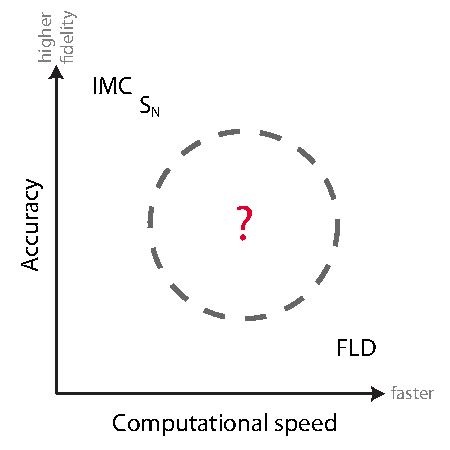
\includegraphics[width=3in]{../figures/fidelity}
\end{center}
% also, storage requirements
\end{frame}
%%%%%%%%%%%%%%%%%%%%%%%%%%%%%%%%%%%%%%%%
\begin{frame}
  \frametitle{Previous work}
  \begin{itemize}
    \item Steady-state VHTR-like problem with analytically calculated
      coefficients \cite{Lar2009c}
    \item Non-local tensor diffusion \cite{Mor2007}, no further development or
      analysis in literature
  \end{itemize}
\end{frame}
%%%%%%%%%%%%%%%%%%%%%%%%%%%%%%%%%%%%%%%%%%%%%%%%%%%%%%%%%%%%%%%%%%%%%%%%%%%%
\section{Theory}
\subsection{Time-dependent linear anisotropic diffusion}
%%%%%%%%%%%%%%%%%%%%%%%%%%%%%%%%%%%%%%%%
\begin{frame}
  \frametitle{Summary in advance}
  \begin{enumerate}
    \item Make assumptions about weakness of derivatives and moments of angular
      flux $\psi(\vec{x}, \vec{\Omega}, t)$: non-rigorous $O(1)$, $O(\epsilon)$.
    \item Substitute the particle conservation equation (zeroth moment of
      Boltzmann equation) into the integral equation for time-dependent angular
      flux.
    \item Apply Taylor series to non-local $\phi$ to get an approximate
      expression for $\psi(\vec{x}, \vec{\Omega}, t)$ as a function of
      $\phi(\vec{x}, t)$ and other problem-dependent quantities.
      Discard $O(\epsilon^2)$ and higher terms.
    \item Take first moment of this approximate $\psi$ to get
      $\vec{J}(\vec{x}, t)$
  \end{enumerate}
\end{frame}
%%%%%%%%%%%%%%%%%%%%%%%%%%%%%%%%%%%%%%%%
\begin{frame}
  Boltzmann transport equation:
  \begin{multline} \label{eq:shortBoltzmannTd}
    \frac1v \pder{\psi}{t}(\vec{x}, \vec{\Omega}, t) + \vec{\Omega} \vd \del
    \psi(\vec{x}, \vec{\Omega}, t) + \Sigma_t (\vec{x}) \psi(\vec{x},
    \vec{\Omega}, t) \\ =
    \frac{1}{4\pi} \left[ \Sigma_s (\vec{x}) \phi(\vec{x}, t) + Q(\vec{x}, t) \right]
  \end{multline}
  Particle conservation by integrating over angles $\int_{4\pi} (\cdot) \ud
  \Omega$:
  \begin{equation} \label{eq:shortConservationTd}
    \frac1v\pder{\phi}{t}(\vec{x}, t) + \del \vd \vec{J}(\vec{x}, t)
    + \Sigma_t (\vec{x}) \phi(\vec{x}, t) =
   \Sigma_s (\vec{x}) \phi(\vec{x}, t) + Q(\vec{x}, t)
  \end{equation}

  \begin{block}{Asymptotic importance ansatz}
    \begin{align*}
      \psi &= O(\epsiloncolor{1}) & \Sigma_t &= O(\epsiloncolor{1}) \\
      \del \psi &= O(\epsiloncolor{\epsilon}) &
      \frac1v\pder{\psi}{t} &= O(\epsiloncolor{\epsilon}) &
      \int_{4\pi} \vec{\Omega} \psi\ud \Omega &= O(\epsiloncolor{\epsilon})
    \end{align*}
  \end{block}
\end{frame}
%%%%%%%%%%%%%%%%%%%%%%%%%%%%%%%%%%%%%%%%
\begin{frame}
  Integral time-dependent transport equation \cite{Pri2010}, neglecting
  boundary and initial conditions:
  \begin{equation} \label{eq:integralAngularFluxShortened}
    \psi(\vec{x}, \vec{\Omega}, t) = 
    \int_{0}^{\infty}
    \eexp^{ - \int_{0}^{s} \Sigma_t(\vec{x}-s'\vec{\Omega}) \ud s'}
    \frac{1}{4\pi}
    \left[ \Sigma_s \phi + Q \right]_{(\vec{x} - s \vec{\Omega}, t-s/v)}
    \ud s
  \end{equation}
  Substituting left hand side of conservation equation,
  Eq.~\eqref{eq:shortConservationTd}:
  \begin{align*}
    \psi(\vec{x}, \vec{\Omega}, t) &= 
    \frac{1}{4\pi} \int_{0}^{\infty}
    \eexp^{ - \tau(\vec{x},\vec{\Omega},s)}
       \left[ \frac1v\pder{\phi}{t} + \del \vd \vec{J}
    + \Sigma_t \phi\right]_{(\vec{x} - s \vec{\Omega}, t-s/v)}
    \ud s
    \\
    \begin{split}
    &= 
    \frac{1}{4\pi} \int_{0}^{\infty} \eexp^{ - \tau(\vec{x},\vec{\Omega},s)}
    \frac1v\pder{\phi}{t}(\vec{x} - s \vec{\Omega}, t-s/v) \ud s
    \\&\qquad + 
    \frac{1}{4\pi} \int_{0}^{\infty} \eexp^{ - \tau(\vec{x},\vec{\Omega},s)}
    \del \vd \vec{J}(\vec{x} - s \vec{\Omega}, t-s/v) \ud s
    \\&\qquad +
    \frac{1}{4\pi} \int_{0}^{\infty} \eexp^{ - \tau(\vec{x},\vec{\Omega},s)}
    \Sigma_t(\vec{x} - s \vec{\Omega}) \phi(\vec{x} - s \vec{\Omega}, t-s/v)
    \ud s
    \end{split}
    \\
    &=
    \underbrace{A}_{O(\epsilon)} + 
    \underbrace{B}_{O(\epsilon^2)} + 
    \underbrace{C}_{O(1)}
  \end{align*}
\end{frame}
%%%%%%%%%%%%%%%%%%%%%%%%%%%%%%%%%%%%%%%%
\begin{frame}
  Taylor series expansion of nonlocal unknowns:
  \begin{align*}
    f(\vec{x} - s \vec{\Omega}, t-s/v)
    &\sim
    f(\vec{x}, t) - s \vec{\Omega} \vd \del f(\vec{x}, t)
    - s\frac{1}{v} \pder{f}{t}(\vec{x}, t) + \cdots
    \\
    &= f(\vec{x}, t) - s \left[ \vec{\Omega} \vd \del
    + \frac{1}{v} \pder{}{t} \right] f(\vec{x}, t) + \cdots
    \\
    &= O(\epsiloncolor{1}) +
    O(\epsiloncolor{\epsilon}) + \cdots
  \end{align*}

  Derivative along streaming direction:
  \begin{align*}
    \oder{}{s} f(\vec{x} - s \vec{\Omega}, t-s/v)
    &=  \oder{}{s} f(x_i - s \Omega_i, t-s/v)
    = \oder{}{s} f(x_1',x_2',x_3',t')
    \\
    &= \sum_{i=1}^{3}
    \pder{x_i'}{s}\pder{x_i}{x_i'} \pder{f}{x_i}
    + \pder{t'}{s}\pder{t}{t'} \pder{f}{t}
    \\
    &= \sum_{i=1}^{3} [- \Omega_i][1]\pder{f}{x_i} 
    + \left( -\frac{1}{v} \right)  \pder{f}{t}
    \\
    &= \left[ -\vec{\Omega} \vd \del f - \pder{f}{t} \right]_{(\vec{x} - s
    \vec{\Omega}, t-s/v)}
  \end{align*}
\end{frame}
%%%%%%%%%%%%%%%%%%%%%%%%%%%%%%%%%%%%%%%%
\begin{frame}
  \frametitle{Properties of anisotropic diffusion}
  \begin{itemize}
    \item
    \item $\Dtens$ are continuous in $\vec{x}$, so anisotropic solution $\phi$
      has continuous first derivatives
    \item Despite smaller cross sections in void regions, propagation speed is
      still infinite
  \end{itemize}<++>
\end{frame}
%%%%%%%%%%%%%%%%%%%%%%%%%%%%%%%%%%%%%%%%%%%%%%%%%%%%%%%%%%%%%%%%%%%%%%%%%%%%
\subsection{Semi-implicit radiative transfer}
%%%%%%%%%%%%%%%%%%%%%%%%%%%%%%%%%%%%%%%%
\begin{frame}
  \frametitle{Thermal radiative transfer equations}
\begin{subequations} \label{eqs:fullGrayTRT}
Radiative transfer equation:
\begin{equation} \label{eq:fullGrayTransport}
  \frac{1}{c} \pder{I}{t}
  + \vec{\Omega} \vd \del I + \textcolor{red}{\sigma} I
  = \frac{\textcolor{red}{\sigma} ac\textcolor{red}{T^4}}{4\pi} 
  + \frac{c Q}{4\pi} \,,
\end{equation}
Material energy balance equation:
\begin{equation} \label{eq:fullGrayMaterial}
  \frac{1}{\textcolor{red}{c_v}}\pder{T}{t} = \textcolor{red}{\sigma} \int_{4\pi}  I \ud
  \Omega - \textcolor{red}{\sigma} ac\textcolor{red}{T^4}
  \,.
\end{equation}
\end{subequations}
\notebox{\textcolor{red}{Red} quantities are temperature-dependent and couple
the material energy to the radiation field.}
\end{frame}
%%%%%%%%%%%%%%%%%%%%%%%%%%%%%%%%%%%%%%%%%%%%%%%%%%%%%%%%%%%%%%%%%%%%%%%%%%%%
\section{Conclusions}
%%%%%%%%%%%%%%%%%%%%%%%%%%%%%%%%%%%%%%%%
\begin{frame}
  \frametitle{Summary}
  \begin{itemize}
    \item Applied transport-calculated coefficients to arbitrary steady-state
      problems
    \item Devised and implemented method to account for diffusion in
      non-orthogonal directions
    \item Time-dependent blah blah
    \item Thermal radiative transport blah blah
  \end{itemize}
\end{frame}
%%%%%%%%%%%%%%%%%%%%%%%%%%%%%%%%%%%%%%%%
\begin{frame}
  \frametitle{Future work}
  \begin{itemize}
    \item Improved time-dependent behavior, with wave propagation speed of $c$
    \item Boundary conditions for both anisotropic diffusion problem and
      purely absorbing transport problem
    \item Improve performance by reducing time spent in transport sweeps
      \begin{itemize}
        \item Evaluate $\Dtens$ on coarser spatial grid, since they are smooth
        \item Update $\Dtens$ less frequently
        \item Advanced quadrature set for \emph{a priori} problem geometry
      \end{itemize}
    \item Quantify the penalty of omitting the $D^{xy}$ terms for various
      problems, or find more effective discretization scheme
  \end{itemize}
\end{frame}
%%%%%%%%%%%%%%%%%%%%%%%%%%%%%%%%%%%%%%%%%%%%%%%%%%%%%%%%%%%%%%%%%%%%%%%%%%%%
\appendix
%%%%%%%%%%%%%%%%%%%%%%%%%%%%%%%%%%%%%%%%
\begin{frame}
  \frametitle{References}
\bibliographystyle{amsalpha}
\bibliography{../SRJall}
\end{frame}
%%%%%%%%%%%%%%%%%%%%%%%%%%%%%%%%%%%%%%%%%%%%%%%%%%%%%%%%%%%%%%%%%%%%%%%%%%%

%	This material is based upon work supported under a National Science
%	Foundation Graduate Research Fellowship. Any opinions, findings, conclusions
%	or recommendations expressed in this publication are those of the author(s)
%	and do not necessarily reflect the views of the National Science
%	Foundation.  
\end{document}
